\documentclass[10pt,twoside]{article}

%
% Use droid mono for fixed-width font
%
\usepackage[defaultmono,scale=0.8]{droidmono}
\usepackage{amsmath,amssymb,amsthm}
\usepackage[subsection]{algorithm}
\usepackage{algpseudocode}
\renewcommand{\algorithmicrequire}{\textbf{Input:}\,}
\renewcommand{\algorithmicensure}{\textbf{Output:}}
\renewcommand{\algorithmicforall}{\textbf{for each}}
\newcommand{\Input}{\Require}
\newcommand{\Output}{\Ensure}
\newcommand{\ForEach}{\ForAll}
\usepackage{graphicx}
\usepackage{caption}
\usepackage{listings}
\lstset{
%  aboveskip=\bigskipamount,
  basicstyle=\ttfamily\small,
%  belowskip=\bigskipamount,
  frame=single,
  language=Python,
  numbers=left,
  numberstyle=\tiny,
  xleftmargin=4pt,
  xrightmargin=4pt
}
\lstnewenvironment{pyoutput}[1][]
{\lstset{aboveskip=-\medskipamount,numbers=none,#1}}
{}



%
% Theorems, Definitions, and Example
%
\theoremstyle{plain}
\newtheorem{theorem}{Theorem}[section]
\newtheorem{lemma}[theorem]{Lemma}
\newtheorem{proposition}[theorem]{Proposition}

\theoremstyle{definition}
\newtheorem{definition}[theorem]{Definition}
\newtheorem{conjecture}[theorem]{Conjecture}
\newtheorem{example}[theorem]{Example}

\numberwithin{equation}{section}

%
% Custom operator declarations
%
\DeclareMathOperator{\ZZ}{\mathbb{Z}}
\DeclareMathOperator{\CC}{\mathbb{C}}
\DeclareMathOperator{\KK}{\mathbb{C}}
\DeclareMathOperator{\PP}{\mathbb{P}}
\DeclareMathOperator{\hh}{\mathfrak{h}}
\DeclareMathOperator{\re}{\text{Re}}
\DeclareMathOperator{\im}{\text{Im}}

%
% Make marginpars smaller font
%
\let\oldmarginpar\marginpar
\renewcommand\marginpar[1]{\oldmarginpar[\scriptsize #1]{\scriptsize #1}}

\newcommand{\thchar}[2] {\begin{bmatrix}#1\\#2\end{bmatrix}}
\newcommand{\thcharsm}[2] {\left[ \begin{smallmatrix} #1 \\ #2 \end{smallmatrix} \right]}

\title{General Examination -- Algebro-Geometric
  Approach to Nonlinear Integrable Equations}

\author{
Chris Swierczewski\\
University of Washington\\
Department of Applied Mathematics}
\date{\today}

%%%%%%%%%%%%%%%%%%%%%%%%%%%%%%%%%%%%%%%%%%%%%%%%%%%%%%%%%%%%%%%%%%%%%%%%%%%%%%%
\begin{document}
%%%%%%%%%%%%%%%%%%%%%%%%%%%%%%%%%%%%%%%%%%%%%%%%%%%%%%%%%%%%%%%%%%%%%%%%%%%%%%%

\maketitle

%%%%%%%%%%%%%%%%%%%%%%%%%%%%%%%%%%%%%%%%%%%%%%%%%%%%%%%%%%%%%%%%%%%%%%%%%%%%%%%
\section{Introduction}
%%%%%%%%%%%%%%%%%%%%%%%%%%%%%%%%%%%%%%%%%%%%%%%%%%%%%%%%%%%%%%%%%%%%%%%%%%%%%%%

The Kadomtsev-Petviashvili (KP) equation is a partial differential
equation used to describe the surface height of a two-dimensional
periodic shallow water wave. Depending on certain physical
considerations [XXX], which we will ignore, one can derive either of the
following two equations
\begin{align}
  \left(-4u_t + 6uu_x + u_{xxx}\right)_x + 3\sigma^2 u_{yy} = 0, \quad
  \sigma^2 = -1, \label{eqn: KP1} \\
  \left(-4u_t + 6uu_x + u_{xxx}\right)_x + 3\sigma^2 u_{yy} = 0, \quad
  \sigma^2 = +1. \label{eqn: KP2}
\end{align}
where $u(x,y,t)$ is the surface height as a function of position $(x,y)$
and time $t$. In the sequel we will not rely on this distinction and
simply refer to the ``KP equation''.

%% \marginpar{
%%   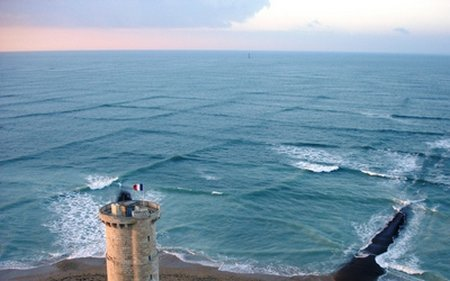
\includegraphics[width=\marginparwidth]{images/livekp.jpg}
%%   \captionof{figure}{KP waves off the coast of \^{I}le de R\'{e}, France.}
%% }

The KP equation admits a large family of quasiperiodic solutions of the
form
\begin{equation} \label{eqn: kpsol}
  u(x,y,t) = 2 \partial_x^2 \log \theta(Ux+Vy+Wt+z_0, \Omega)
\end{equation}
where $\theta$ is the Riemann theta function.

\begin{definition} \label{def: riemanntheta}
  The {\bf Riemann theta function} $\theta: \CC^g \times \hh_g \to \CC$
  is defined in terms of its Fourier series
  \begin{equation} \label{eqn: riemanntheta}
    \theta(z,\Omega) = \sum_{n \in \ZZ^g}
    e^{2 \pi i \left( \tfrac{1}{2} n \cdot \Omega n + n \cdot z \right)}.
  \end{equation}
  $\theta$ converges absolutely and uniformly on compact sets in $\CC^g
  \times \hh_g$ where $\hh_g$ is the space of all {\it ``Riemann
    matrices''} --- complex symmetric matrices with positive definite
  imaginary part.
\end{definition}

From the definition, we see that the Riemann theta function is periodic
in $z$ with integer periods and quasi-periodic in $z$ in the columns of
$\Omega$. In other words, if $m,n \in \ZZ^g$ then
\begin{equation} \label{eq: quasiperiodicity}
    \theta(z + m + \Omega n, \Omega) =
    e^{-2 \pi i \left( \tfrac{1}{2} n \cdot \Omega n + n \cdot z \right) }
    \theta(z, \Omega).
\end{equation}

A generalization of the Riemann theta function, involving a non-integer
shift in some of its arguments, is referred to as the Riemann theta
function with characteristics.

\begin{definition} \label{def: thetachar}
Let $\alpha,\beta \in [0,1)^{g}$. The {\bf Riemann theta function with
characteristic $\thcharsm{\alpha}{\beta}$} is defined as
\begin{align*}
  \theta\thchar{\alpha}{\beta}(z, \Omega) &=
  \sum_{n \in \mathbb{Z}^g}
  e^{2 \pi i \left( \tfrac{1}{2} (n+\alpha) \cdot \Omega (n+\alpha) +
    (n + \alpha) \cdot (z + \beta) \right) } \\
  &=
  e^{2\pi i \left( \tfrac{1}{2} \alpha \cdot \Omega \alpha +
    \alpha \cdot (z + \beta) \right)}
  \theta(z + \Omega \alpha + \beta, \Omega).
\end{align*}
\end{definition}

Note that $\theta \thcharsm{0}{0}(z,\Omega) = \theta(z,\Omega)$. See
\cite{DLMF,MumfordI07,MumfordII07} for further definitions and
properties of the Riemann theta function.

Returning to Equation \eqref{eqn: kpsol}, these solutions are the
so-called ``theta function solutions'' to the KP equation and families
of such solutions exist for every $g > 0$. In fact, the totality of
solutions of this form are dense the space of all periodic solutions to
KP. [XXX Marchenko and Ostrovskii?, see Dubrovin] The constants
$U,V,W,z_0 \in \CC^g$ and $\Omega \in \hh_g$, as well as the ``genus''
$g$, are all determined from a Riemann surface corresponding to a
complex plane algebraic curve $f \in \CC[x,y]$ and any such curve can
produce a solution to KP. \cite{Dubrovin81} We will postpone the
definition of these constants in terms of known quantities until more
machinery is developed in the following chapters.

\marginpar{Improve / elaborate upon the role of Abelian functions. This
  paragraph is a bit...I dunno.}

In general, periodic solutions to partial differential equations are
Abelian functions: doubly-periodic meromorphic functions defined on
Riemann surfaces [XXX]. Riemann theta functions play a central role in
the theory of Abelian functions in that all Abelian functions can be
written as a rational function of the Riemann theta function and its
derivatives. (Such as in the KP solution above.) Therefore, a primary
focus of study is the method of computation of these Abelian functions.

The theory of Riemann theta functions and algebraic curves is applicable
to solving problems in fields other than nonlinear partial differential
equations. For example Riemann theta functions are involved in the
computation of bitangent lines; useful for computations in
optimization-related fields such as algebraic geometry and convex
optimization. In algebraic geometry, bitangents can represent smooth
complex plane quartic curves as both a symmetric determinant of a linear
form (or, determinantal representation) as well as a sum of three
squares. \cite{PSV11} In convex optimization, bitangents are used to
construct a ``visibility complex'' which, in turn, is used to solve the
shortest path problem in Euclidean space \cite{PocchiolaVegter93}

\begin{definition} \label{def: bitangent}
  A {\bf bitangent} to a plane algebraic curve $C : f(x,y) = 0, f \in
  \CC[x,y]$ is a line $\mathcal{L} \subset \CC$ that lies tangent to $C$
  at at least two distinct points.
\end{definition}

By Bezout's Theorem, if a curve has a bitangent it necessarily must be
of degree at least four. \cite{Bezout1779} A result of Pl\"{u}cker
determines that a degree four complex curve admits exactly 28 complex
bitangents. \cite{Plucker34} In particular, Pl\"{u}cker showed that the
number of real bitangents of any quartic must be 28, 16, or fewer than
9. The connection between Riemann theta functions and the bitangent
lines of smooth quartics was known to Riemann \cite{Riemann76} and, in
fact, can be computed using the tools developed in this research. See
Figure \ref{fig: edge} for an example.

\marginpar{Note: Figure \ref{fig: edge} will be replaced with the one
  generated by abelfunctions once I have it working properly again /
  once I find the image on my computer.}

\begin{figure}[t]
  \centering
  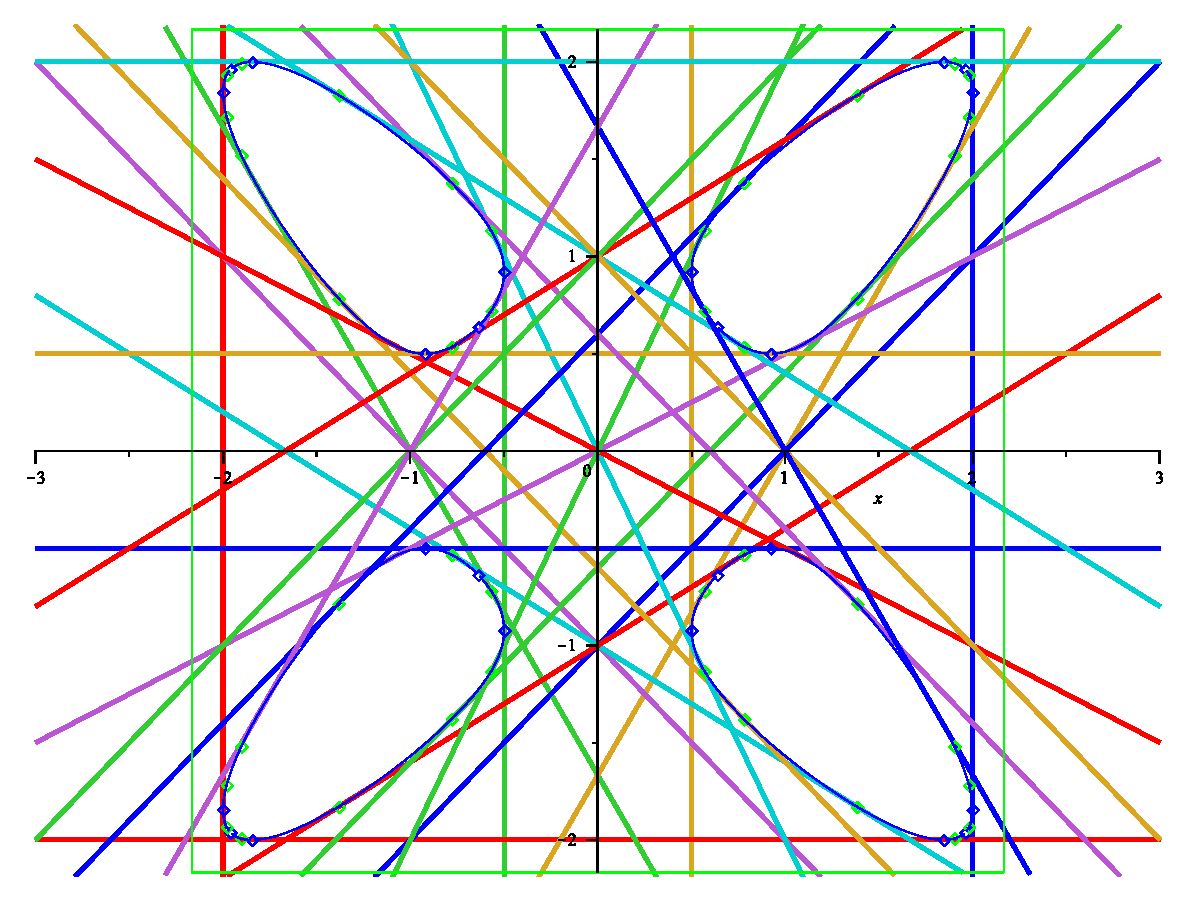
\includegraphics[width=0.8\textwidth]{images/edgequartic}
  \caption{The real graph of the Edge Quartic $C: f(x,y) = 25(x^4+y^4+1)
    - 34(x^2y^2+x^2+y^2) = 0$ and its 28 real bitangents. Note that four
    of them lie tangent $C$ at infinity. These lines were computed using
    the Riemann theta function.}
  \label{fig: edge}
\end{figure}

Finally, Riemann theta functions and algebraic curves can be used to
compute linear matrix representations of algebraic curves. A theorem
from classical algebraic geometry states that every homogenous
polynomial $f \in P^2\CC[x_0,x_1,x_2]$ can be written in the form
\[
   f(x_0,x_1,x_2) = \text{det}
   \left( A x_0 + B x_1 + C x_2 \right)
\]
where $A,B,C$ are symmetric complex matrices which can be efficiently
computed using Riemann theta functions. Furthermore, when the polynomial
has real coefficients then $A,B,C$ are symmetric real matrices and such
representations are important in the study of spectrahedra --- the
solution spaces of semidefinite programs. \cite{PSV10}

The purpose of this research is to develop efficient and performant
algorithms for computing with Abelian functions on Riemann surfaces. The
computational tools developed in this research program have far-reaching
and varied applications.


%%%%%%%%%%%%%%%%%%%%%%%%%%%%%%%%%%%%%%%%%%%%%%%%%%%%%%%%%%%%%%%%%%%%%%%%%%%%%%%
\section{Complex Algebraic Geometry --- Period Matrices and the Abel Map}
%%%%%%%%%%%%%%%%%%%%%%%%%%%%%%%%%%%%%%%%%%%%%%%%%%%%%%%%%%%%%%%%%%%%%%%%%%%%%%%

In this section we give a brief introduction to the theory of complex
algebraic curves. We explain the concept of a period matrix and the Abel
map, a particular function from a Riemann surface to the complex
numbers.

%..............................................................................
\subsection{Projective Space and Projective Curves}
%..............................................................................

We begin with an introduction to complex projective geometry. The point
of the construction is to make concrete the way in which we analyze the
behavior of functions, such as polynomials, at infinity without having
to resort to techniques separate from those used at finite points.

In fact, one with an elementary complex analysis background will have
already seen an example of projective geometry. The Riemann sphere is
the complex plane $\CC$ with a ``point at infinity'' added. If $z$ is
the coordinate in $\CC$ then $w = 1/z$ is the coordinate around the
point at infinity. This explains why, for example, the exponential
function
\[
    e^z = \sum_{n=0}^\infty z^n / n!
\]
has an essential singularity at infinity because, in the coordinate $w$
at infinity, the exponential function is expressed by the series
\[
    \sum_{n=0}^\infty w^{-n} / n!.
\]

The definition of the Riemann sphere is made explicit by the following
construction: consider the set $U = \CC^2 - \{(0,0)\}$. Define the
equivalence relation
\[
    (a_0, a_1) \sim (\lambda a_0, \lambda a_1),
    \quad \forall \lambda \neq 0.
\]
This is equivalent to saying that all ratios $a_0 : a_1$ are considered
equivalent points in $U$. The {\it complex projective line} $P^1\CC$ is
the set of all such equivalence classes. That is,
\[
    P^1\CC := \CC^2 / \sim.
\]
Points in $P^1\CC$ are typically written as $(a_0 : a_1)$.

The claim is that $P^1\CC$ is precisely the Riemann sphere. Consider the
two subsets
\begin{align*}
    U_0 &= \{ (a_0 : a_1) \in P^1\CC \; | \; a_0 \neq 0 \}, \\
    U_1 &= \{ (a_0 : a_1) \in P^1\CC \; | \; a_1 \neq 0 \}.
\end{align*}
For any $(a_0 : a_1) \in U_0$ we have, by the equivalence property,
\[
    (a_0 : a_1) = (1 : a_1/a_0) = (1 : a).
\]
Similarly, every point $(b_0 : b_1) \in U_1$ can be written as $(b : 1)$
and in the intersection $U_0 \cap U_1$ every element can be written in
either of these two forms.

Each of these subspaces are isomorphic to $\CC$ since the maps $\phi_0 :
(a_0 : a_1) \in U_0 \mapsto a_1 / a_0 \in \CC$ and $\phi_1 : (a_0 : a_1)
\in U_1 \mapsto a_0 / a_1 \in \CC$ are continuous bijections with
inverses $\phi^{-1}_0 : a \in \CC \mapsto (1 : a) \in U_0$ and
$\phi^{-1}_1 : b \in \CC \mapsto (b : 1) \in U_1$.

Which points in $P^1\CC$ remain? Note that the point $(1 : 0) \in U_0$



%------------------------------------------------------------------------------
\subsection{Introduction to Algebraic Curves}
%------------------------------------------------------------------------------

Primary references. \cite{Griffiths89, Ueno97}

A complex plane algebraic curve, $C$, is the zero locus of the
homogenization of a polynomial $f \in \CC[x,y]$. That is, given a
polynomial $f(x,y) = a_n(x) y^n + a_{n-1}(x)y^{n-1} + \cdots + a_0(x)$
its homogenization is the polynomial $F \in P^2\CC[x_0,x_1,x_2]$ where
\[
  F(x_0,x_1,x_2) = x_0^d f(x_1/x_0,x_2/x_0).
\]
where $d$ is the degree of $F$ and $P^2\CC$ denotes two-dimensional
complex projective space. We often consider the {\it affine curve}
$f(x,y) = F(1,x,y)$, which can be thought of as a projection of the
curve $F$ to $\CC^2[x,y]$. Therefore, a {\it complex plane algebraic
  curve} is the set
\[
  C = \left\{
  (x_0 : x_1 : x_2) \in P^2\CC : F(x_0,x_1,x_2) = 0
  \right\}.
\]

%..............................................................................
\subsubsection*{Singular Points}
%..............................................................................

A point $p = (a_0 : a_1 : a_2) \in C$ is a {\it singular point of $C$},
or a {\it multiple point of $C$}, if
\[
  \left(
    \frac{\partial F}{\partial x_0} (p),
    \frac{\partial F}{\partial x_1} (p),
    \frac{\partial F}{\partial x_2} (p)
  \right)
  = 0.
\]
Just as with roots, singular points have a multiplicity. Without loss of
generality we consider the case when $p = (1 : 0 : 0)$ is a singular
point of $F$. The corresponding affine curve is $f(x,y) = F(1,x,y)$
which we write as
\[
  f(x,y) = \sum_{i+j \geq 2}^d a_{ij} x^iy^j.
\]
Note that the constant term is zero since we've centered the curve at
$(0, 0)$, a point of the affine curve, and the linear term vanishes
since $(0,0)$ is a singular point. We then write
\[
  f(x,y) = f_m(x,y) + f_{m+1}(x,y) + \cdots + f_d(x,y), \quad m \geq 2
\]
where each $f_n$ is the sum of all of the terms of $f$ of degree $n$;
that is, terms of the form $a_{ij}x^iy^j$ such that $i+j=n$. The
smallest such $m$ with non-zero term $f_m$ appearing in $f$ is called
the {\it multiplicity} of the singular point $(1 : 0 : 0)$. This
homogenous term can be factored into linear factors
\[
  f_m(x,y) = \prod_{j=1}^m (\alpha_jx - \beta_jy).
\]
We call the space $f_m(x,y) = 0$ the {\it tangent cone of the plane
  curve $C$} at $(1 : 0 : 0)$, which consists of a finite number of
lines.

If the singular point $p$ is elsewhere we can simply map the singular
point to $(1 : 0 : 0)$ via projective transformation. It is also
possible to deal with the case directly. If $p = (1 : a : b)$ is a
singular point then we write the affine curve in the form
\[
    f(x,y) = \sum_{i+j \geq 2}^d a_{ij} (x-a)^i(y-b)^j
\]
and then write as a sum of homogenous polynomials $g_n(x-a,y-b)$. In the
case when the singular point is $p = (0 : 1 : b)$ we repeat the above
process with the affine curve $g(u,v) = F(u,0,v)$ centered at
$(0,b)$. Finally, the case $p = (0 : 0 : 1)$ [XXX]

\begin{example}
Let us consider the cubic curve
\[
    C: F(x_0,x_1,x_2) = x_0x_1^2 + x_1^3 - x_2^2x_0 = 0.
\]
For $p = (a_0 : a_1 : a_2)$ we have
\begin{align*}
    \Delta_x^1 F(a) &=
        (a_1^2 - a_2^2)x_0 + a_1(2a_0 + 2a_1)x_2 - 2a_0a_2x_2 \\
    \Delta_x^2 F(a) &=
        4a_1x_0x_1 + 2(a_0+3a_1)x_1^2 - 2a_0x_2^2 - 4a_2x_2x_0.
\end{align*}
Note that the point $a = (1 : 0 : 0)$ satisfies $\Delta_x^1 F(a) \equiv
0$ and $\Delta_x^2 F(a) \not \equiv 0$. The tangent cone at $a$ is given
by
\[
    \Delta_x^2 F(a) = x_1^2 - x_2^2 = 0
\]
which represents two lines $x_1 - x_2 = 0$ and $x_1 + x_2 = 0$. When the
tangent cone at $a$ can be completely factored into linear terms we say
$a$ is an {\it ordinary} double point of the curve, $C$. On the affine
plane $x_0=1$, equivalent to setting $x = x_1/x_0$ and $y=x_2/x_0$, this
gives the curve $f(x,y) = y^3 + xy^2 - x$. In Figure \ref{fig:
  double-pt-example} we see the double-point singularity appearing at
the origin where two ``branches'' of the curve meet.
\end{example}

\begin{figure}
  \label{fig: double-pt-example}
  \caption{A real plot of the curve $f(x,y) = y^3 + xy^2 - x$ in the $x-y$ plane.}
\end{figure}

%------------------------------------------------------------------------------
\subsection{Connection to Riemann Surfaces}
%------------------------------------------------------------------------------

There exists a close relationship between the study of compact Riemann
surfaces and that of algebraic curves. A Riemann surface $\tilde{C}$ is
simply a complex manifold of complex dimension one. This relationship is
embodied by the following two theorems.

\begin{theorem} \label{thm: normalization}
  {\it (Normalization Theorem.)} For any irreducible algebraic curve $C
  \subset P^2\CC$ there exists a compact Riemann surface $\tilde{C}$ and
  a holomorphic mapping
  \[
    \sigma : \tilde{C} \to P^2\CC
  \]
  such that $\sigma( \tilde{C} ) = C$ adn $\sigma$ is injective on the
  inverse image of the set of smooth points of $C$.
\end{theorem}

A Riemann surface together with the mapping $\sigma$ is called the {\it
  normalization of $C$}. Loosely speaking, the normalization theorem
states that an algebraic curve is a Riemann surface except at the
singular points.

%% In particular, any irreducible plane algebraic curves admits a
%% holomorphic parametric representation and the domain of definition of
%% this representation is a compact Riemann surface [[[]]]. The following
%% two theorems indeed show




%%%%%%%%%%%%%%%%%%%%%%%%%%%%%%%%%%%%%%%%%%%%%%%%%%%%%%%%%%%%%%%%%%%%%%%%%%%%%%%
\section{Computing Period Matrices of Algebraic Curves and the Abel Map}
%%%%%%%%%%%%%%%%%%%%%%%%%%%%%%%%%%%%%%%%%%%%%%%%%%%%%%%%%%%%%%%%%%%%%%%%%%%%%%%

In this section we will look at algorithmically computing period
matrices. Each subsection here examines in close detail a major
component of the algorithm and provides a theoretical overview of the
component, an algorithm for computing the component, and an example
presented in {\tt abelfunctions}, a Python software package


%------------------------------------------------------------------------------
\subsection{abelfunctions}
%------------------------------------------------------------------------------

%------------------------------------------------------------------------------
\subsection{Puiseux Series}
%------------------------------------------------------------------------------

%..............................................................................
\subsubsection*{Theory}
%..............................................................................

%..............................................................................
\subsubsection*{Algorithm}
%..............................................................................

\begin{algorithm}[h]
\caption{POLYGON --- Returns the Newton polygon of the polynomial $F =
  F(X,Y)$.}
\label{alg: puiseux-polygon}
\begin{algorithmic}[1]
\Input

$F,X,Y$ --- A polynomial.

$I$ --- If $I=0$, return the Newton polygon. If $I=1$, return only the
segments of the Newton polygon with negative slope. $I=1$ is used to
compute terms beyond the first of the Puiseux series.

\Output A set of lists $(q,m,l,\Phi)$ where
\begin{itemize}
  \item $q,m,l$ defines a line segment $\Delta: qj+mi=l$ in the $(i,j)$
    plane,
  \item $\Phi(Z) = \sum_{(i,j)\in\Delta} a_{ij} Z^{(i-i_0)/q} \in
    \CC[Z]$ where $i_0$ is the smallest value of $i$ such that there is
    a point $(i_0,j)\in\Delta$.
\end{itemize}

\Function{POLYGON}{$F,X,Y,I$}
  \State
\EndFunction
\end{algorithmic}
\end{algorithm}


\begin{algorithm}[h]
\caption{REGULAR --- Given the branching or singular part of a Puiseux
  series, computes the regular part of the series.}
\label{alg: puiseux-regular}
\begin{algorithmic}[1]
\Input

$S$ --- a finite set of pairs $\{(\pi_k,F_k)\}$

$X,Y$ --- the dependent and independent variables, respectively

$H$ --- bound on the number of desired terms of the series

\Output $R$ --- a finite set of pairs $\{(\pi_k,F_k)\}$ containing at
least $H$ terms

\Function{Regular}{$S,X,Y,H$}
  \State $R \leftarrow ()$
  \ForEach{$(\pi,F)$ {\bf in} $S$}
    \While{$\text{len}(\pi) < H$}

      \State $m \leftarrow \text{min} \{ j \; /$
      \Call{COEFFICIENT}{$F,0,j$} $ \; | \; j \neq 0 \}$

      \State $\beta \leftarrow$ \Call{COEFFICIENT}{$F,0,m$} /
      \Call{COEFFICIENT}{$F,1,0$}

      \State $\tau \leftarrow (1,1,m,\beta)$
      \State $\pi \leftarrow \pi \cup \{\tau\}$
      \State $F \leftarrow$ \Call{NEWPOLYNOMIAL}{$F,\tau,m$}
    \EndWhile
    \State $R \leftarrow R \cup \{\pi\}$
  \EndFor
\EndFunction
\end{algorithmic}
\end{algorithm}

%..............................................................................
\subsubsection*{Examples}
%..............................................................................

\begin{lstlisting}
from abelfunctions import *
from sympy.abc import x,y,t

alpha = 0
f = y**8 + x*y**5 + x**4 - x**6
C = RiemannSurface(f,x,y)
p = C.puiseux(alpha, nterms=3, parametric=t)

for pi in p:
    sympy.pprint(pi)
\end{lstlisting}
\begin{pyoutput}
          11    7      
  5    6*t     t     3 
(t , - ----- - -- - t )
         25    5       
           9    5     
   3    2*t    t      
(-t , - ---- - -- + t)
         3     3      
\end{pyoutput}

%------------------------------------------------------------------------------
\subsection{Singularities}
%------------------------------------------------------------------------------

%
\subsubsection*{Theory}
%
%
\subsubsection*{Algorithm}
%
%
\subsubsection*{Examples}
%

%------------------------------------------------------------------------------
\subsection{Holomorphic Differentials}
%------------------------------------------------------------------------------

%
\subsubsection*{Theory}
%



%
\subsubsection*{Algorithm}
%
%
\subsubsection*{Examples}
%

%------------------------------------------------------------------------------
\subsection{Analytic Continuation}
%------------------------------------------------------------------------------

%
\subsubsection*{Theory}
%

A path on a Riemann surface is a continuous map $\gamma : [0,1] \to C
\subset \CC^2$. That is, if $\gamma(t) = (x_\gamma(t), y_\gamma(t))$
then $f(x(t),y(t)) = 0$ for all $t \in [0,1]$.


%
\subsubsection*{Algorithm}
%

Since analytic continuation is repeatedly performed when computing
period matrices it is important to make it performant.

Often, a path in $\CC_x$, $x_\gamma$, will be specified, such as via the
{\sc monodromy() or homology()} functions, and the corresponding
$y$-values lying above need to be determined. A naive approach to doing
so is to use a numerical root finder.

An alternate approach, which is the one used here, is to use Newton's
method --- given $x_\gamma(t_k)$ and some $y_{\gamma,j}(t_k)$ lying
above determine $y_{\gamma,j}(t_{k+1})$ above $x_\gamma(t_{k+1})$.

%
\subsubsection*{Examples}
%

%------------------------------------------------------------------------------
\subsection{Monodromy}
%------------------------------------------------------------------------------

%
\subsubsection*{Theory}
%
%
\subsubsection*{Algorithm}
%
%
\subsubsection*{Examples}
%

%------------------------------------------------------------------------------
\subsection{Homology}
%------------------------------------------------------------------------------

%
\subsubsection*{Theory}
%
%
\subsubsection*{Algorithm}
%
%
\subsubsection*{Examples}
%

%------------------------------------------------------------------------------
\subsection{Period Matrices}
%------------------------------------------------------------------------------

%
\subsubsection*{Theory}
%
%
\subsubsection*{Algorithm}
%
%
\subsubsection*{Examples}
%

%------------------------------------------------------------------------------
\subsection{The Abel Map}
%------------------------------------------------------------------------------

%
\subsubsection*{Theory}
%
%
\subsubsection*{Algorithm}
%
%
\subsubsection*{Examples}
%

%%%%%%%%%%%%%%%%%%%%%%%%%%%%%%%%%%%%%%%%%%%%%%%%%%%%%%%%%%%%%%%%%%%%%%%%%%%%%%%
\section{Periodic Solutions to Nonlinear Integrable Equations}
%%%%%%%%%%%%%%%%%%%%%%%%%%%%%%%%%%%%%%%%%%%%%%%%%%%%%%%%%%%%%%%%%%%%%%%%%%%%%%%

%------------------------------------------------------------------------------
\subsection{Example: The Kadomtsev--Petviashvili Equation}
%------------------------------------------------------------------------------

%------------------------------------------------------------------------------
\subsection{Geometry of Integrable Equations}
%------------------------------------------------------------------------------


%%%%%%%%%%%%%%%%%%%%%%%%%%%%%%%%%%%%%%%%%%%%%%%%%%%%%%%%%%%%%%%%%%%%%%%%%%%%%%%
\section{Future Work}
%%%%%%%%%%%%%%%%%%%%%%%%%%%%%%%%%%%%%%%%%%%%%%%%%%%%%%%%%%%%%%%%%%%%%%%%%%%%%%%

%------------------------------------------------------------------------------
\subsection{Periodic Solutions of Integrable Equations}
%------------------------------------------------------------------------------

%------------------------------------------------------------------------------
\subsection{Fay's Prime Form}
%------------------------------------------------------------------------------

%------------------------------------------------------------------------------
\subsection{The Constructive Schottky Problem}
%------------------------------------------------------------------------------


%%%%%%%%%%%%%%%%%%%%%%%%%%%%%%%%%%%%%%%%%%%%%%%%%%%%%%%%%%%%%%%%%%%%%%%%%%%%%%%
\section{Bibliography}
%%%%%%%%%%%%%%%%%%%%%%%%%%%%%%%%%%%%%%%%%%%%%%%%%%%%%%%%%%%%%%%%%%%%%%%%%%%%%%%


\bibliographystyle{amsalpha}
\bibliography{general-exam}


%%%%%%%%%%%%%%%%%%%%%%%%%%%%%%%%%%%%%%%%%%%%%%%%%%%%%%%%%%%%%%%%%%%%%%%%%%%%%%%
\end{document}
%%%%%%%%%%%%%%%%%%%%%%%%%%%%%%%%%%%%%%%%%%%%%%%%%%%%%%%%%%%%%%%%%%%%%%%%%%%%%%%
